\chapter{论文的初始化}
\label{chp:initialization}

在开始撰写学位论文之前,我们建议你首先对你论文的基本信息进行初始化。这部分的工作在main.tex文件中完成。接下来我们将详细介绍各部分的填写方法。注意,下列所有源代码中尖括号{\codefont <...>}里的内容代表你需要填写的文本。

\section{元数据}

元数据部分控制你论文A3封面和中文彩色封面左上角的论文元信息的显示,除固定的学校代码外分为4个部分。下面我们将逐一解释每个部分的填写规则。

\subsection{分类号}

分类号指代中国图书馆分类法 (CLC, Chinese Library Classification)对图书资料的分类编码,请根据你学术论文的内容与分类酌情填写。

\begin{tcolorbox}
\begin{lstlisting}[language=TeX]
\categorynumber{<CLC Code>}
\end{lstlisting}
\end{tcolorbox}

\noindent 举例来说,\textbf{网络安全}的中图法分类号为TN915.08,而\textbf{建筑水利工程}的分类号为F407.9。如对自己研究内容的具体分类不甚确定,可以参阅\href{https://www.clcindex.com/}{相关网站}。

\subsection{UDC}

UDC(Universal Decimal Classification)指通用十进制分类法,是国际上规模最大影响最广泛的文献资料分类法。在此部分你需要填写学术论文所属的十进制分类编码。

\begin{tcolorbox}
\begin{lstlisting}[language=TeX]
\UDC{<UDC Code>}
\end{lstlisting}
\end{tcolorbox}

\noindent 举例来说,\textbf{人工智能}的UDC分类号为004.8,而\textbf{凝聚态固态物理学}的分类号为538.9。如对自己研究内容的具体分类不甚确定,可以参阅\href{http://www.udcsummary.info/php/index.php?lang=chi}{相关网站}。

\subsection{保密级别}

在此部分你需要指定你的学术论文所属的保密级别。

\begin{tcolorbox}
\begin{lstlisting}[language=TeX]
\secretlevel{<Secret Level>}
\end{lstlisting}
\end{tcolorbox}

\noindent 一般的,学位论文的保密级别分为公开、内部、秘密和机密四级。具体区别在于:

\begin{itemize}
  \item \textbf{公开}:未涉及国家保密范围以及未准备申请专利权或技术转让的一般学术研究;
  \item \textbf{内部}:未涉及国家保密范围但准备申请专利权或技术转让的在一段时间内不适宜公开的学术研究;
  \item \textbf{秘密与机密}:涉及国家保密特定密级的科研项目或课题及其衍生的学术研究。
\end{itemize}

\noindent 请根据你的论文的具体情况酌情填写。

\subsection{学号}

在此部分你需要填写你的研究生学号。

\begin{tcolorbox}
\begin{lstlisting}[language=TeX]
\studentid{<Student ID>}
\end{lstlisting}
\end{tcolorbox}

\noindent 东南大学的研究生学号一般为6位数字,请注意不要与9位的一卡通号混淆。也请学号为8位数字的本科生同学关闭本文档,出门左转GitHub寻找适合本科生的论文模板。

\section{论文标题与书脊}

\subsection{中英文标题}

论文标题部分控制你论文的A3封面、中文彩色封面、中文内页封面和英文封面上的标题显示。

\begin{tcolorbox}
\begin{lstlisting}[language=TeX]
\title
    {弯扭耦合下土木工程复合材料梁的变分渐近模型}
    {}
    {Variational Asymptotic Model of Composite Beams Used in Civil Engineering under Bending and Torsion Coupling}
    {}
\end{lstlisting}
\end{tcolorbox}

\noindent 对论文标题的指定分为4个部分,自上而下分别是中文主标题,中文副标题,英文主标题和英文副标题。对于大多数没有副标题的学位论文,中英文副标题部分可以留空,但请务必不要删去相应的括号。有些论文的中英文标题可能过长,这时你也可以使用副标题位置来实现更加灵活自主的换行。比如上面的示例可以改写成:

\begin{tcolorbox}
\begin{lstlisting}[language=TeX]
\title
    {弯扭耦合下土木工程复合材料梁}
    {的变分渐近模型}
    {Variational Asymptotic Model of Composite Beams Used in Civil}
    {Engineering under Bending and Torsion Coupling}
\end{lstlisting}
\end{tcolorbox}

\noindent 当你把主标题的后半部分拆分并写到副标题中时,\LaTeX 编译引擎会尝试在你拆分的位置换行。但想要做到这一点需要耐心调整拆分位置,否则如果你的上半部分仍然过长,编译时会被拆分成三行。

\subsection{论文书脊}

论文书脊指出现在A3封面垂直中间部分的文章标题及作者姓名,在论文装订时将被作为书册的书脊。对于大多数学术论文,作者不需要特地显式地声明书脊部分,本模板将会直接利用你的中文标题生成书脊。但如果你的中文标题中出现了英文或其他语言的拉丁字母,直接使用标题生成书脊将会出现图 \ref{fig:2_1} 所显示的问题:

\begin{figure}[!h]
  \centering
    \begin{minipage}[t]{0.48\textwidth}
    \centering
    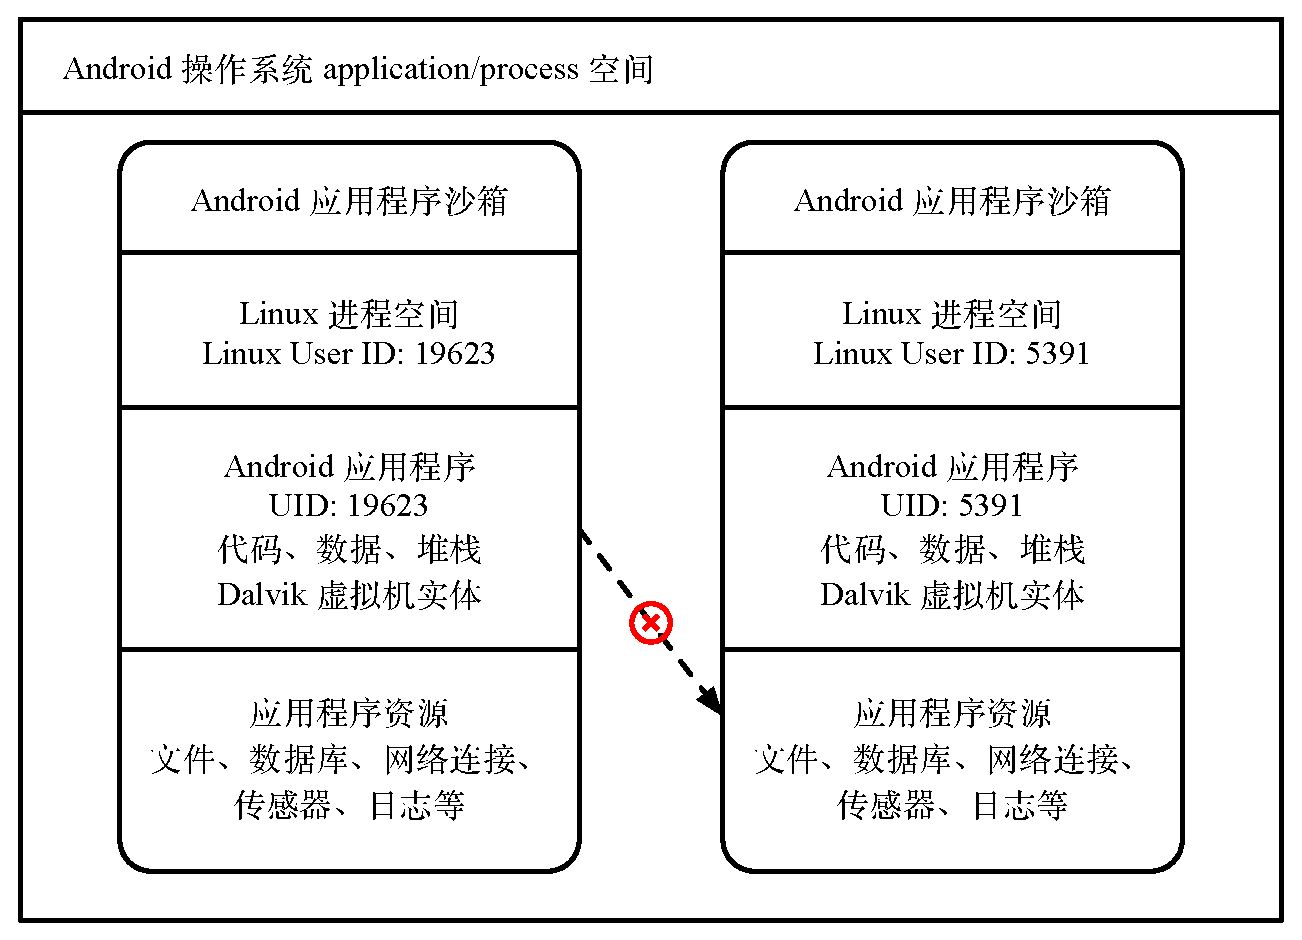
\includegraphics[width=.3\linewidth]{figures/content/2_1}
    \caption{错误的书脊渲染}
    \label{fig:2_1}
    \end{minipage}
    \begin{minipage}[t]{0.48\textwidth}
    \centering
    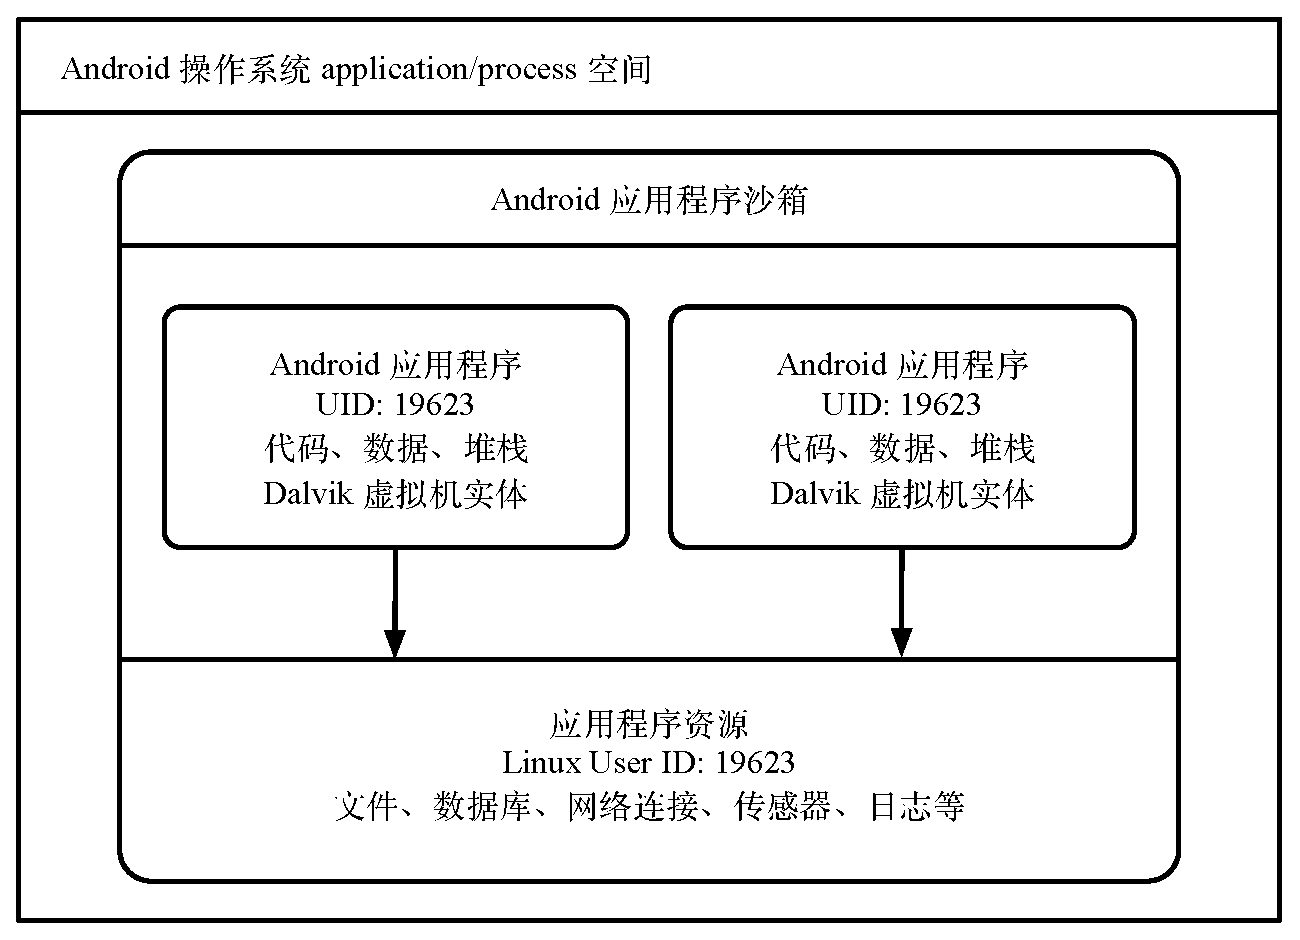
\includegraphics[width=.3\linewidth]{figures/content/2_2}
    \caption{正确的书脊渲染}
    \label{fig:2_2}
    \end{minipage}
\end{figure}

\noindent 这时你必须显式地指定书脊的渲染方式。指定的方式很简单,你只需告知编译引擎对标题中的西文字母进行逆时针270$^{\circ}$(即顺时针90$^{\circ}$)旋转即可:

\begin{tcolorbox}
\begin{lstlisting}[language=TeX]
\spine
    {面向种群的 \rotatebox{270}{Android} 安全风险评估和恶意应用检测}
    {}
\end{lstlisting}
\end{tcolorbox}

\noindent 请注意,{\codefont $\backslash$rotatebox\{270\}\{\}}前后应该各留一个空格,否则会导致编译错误。和论文标题类似,没有副标题时上述第2个字段可以留空。这样修正后的书脊渲染如图 \ref{fig:2_2} 所示。再次强调,如果你的论文标题中没有中西文混排,请直接删去{\codefont $\backslash$spine}字段。

\section{作者与导师}

该部分用于指定论文的作者与导师姓名。作者字段分为2个部分,分别是作者的中文名及其拉丁文转写:

\begin{tcolorbox}
\begin{lstlisting}[language=TeX]
\author
    {陈仁营}
    {CHEN Ren-ying}
\end{lstlisting}
\end{tcolorbox}

\noindent 关于中文姓名转写为英文时的拼写规则,根据《东南大学研究生学位论文格式规定》\cite{seugs2015rule}第一条第二款之要求,有如下规定:

~

\noindent{\color{black!45}
中国姓名译为英文时用汉语拼音,按照姓前名后的原则,姓、名均用全名,不宜用缩写。姓全用大写,名的第一个字母大写,名为双中文字时两个字的拼音之间可以不用短划线,但容易引起歧义时必须用短划线。例如“冯长根”译为“FENG Changgen”或“FENG Chang-gen”,而“冯长安”则必须译为“FENG Chang-an”。论文英文封面上的署名也遵守此规定。}

~

导师字段分为3个部分,分别是导师的中文名、姓名的拉丁文转写以及导师的英文职称,用于显示在英文封面上:

\begin{tcolorbox}
\begin{lstlisting}[language=TeX]
\advisor
    {张广军}
    {ZHANG Guang-Jun}
    {Prof.}
\end{lstlisting}
\end{tcolorbox}

\noindent 对于硕士研究生和博士研究生,导师的职称一般为副教授级及以上。导师为副教授的,职称可以写全称 Associate Professor,也可以写简称 A. Prof.;导师为教授的,可以写全称 Professor或简称Prof.,注意上述简称中的~.不可省略。对于导师职称未达副教授级的特殊情况,比如导师职称为讲师时,请勿在职称处填写Lecturer,此时宜填写Doctor或Dr.以示尊重。

一些硕士研究生可能会有副导师,此时可以显式指定副导师的相关信息,具体方法和导师相同:

\begin{tcolorbox}
\begin{lstlisting}[language=TeX]
\coadvisor
    {程光}
    {CHENG Guang}
    {Prof.}
\end{lstlisting}
\end{tcolorbox}

\noindent 没有副导师的研究生学位论文,请删去上述几行。

\section{答辩信息}

答辩信息用于在论文A3封面和中文彩色封面中渲染与研究生论文答辩相关的信息。

\begin{tcolorbox}
\begin{lstlisting}[language=TeX]
\degreetype{工学硕士}{Master of Engineering}
\major{生物医学工程}
\submajor{神经信息工程}
\defenddate{2020年1月20日}
\authorizedate{2020年1月23日}
\committeechair{齐康}
\reviewer{王建国}{韩冬青}
\department{网络空间安全学院}{School of Cyberspace Security}
\seuthesisthanks{本文的部分工作受国家自然基金 No. wdnmd666 的支持与帮助,在此表示感谢。}
\end{lstlisting}
\end{tcolorbox}

其中,{\codefont degreetype}字段用于指定所申请的学位类型与等级。{\codefont major}和{\codefont submajor}字段用于指定研究生攻读的一级和二级学科名称,请依照中华人民共和国教育部一级和二级学科名录进行填写。如果所属专业直接隶属于一级学科,{\codefont submajor}字段可以留空不填。{\codefont defenddate}和{\codefont authorizedate}分别用于指定论文的答辩日期和学位的授予日期,请根据实际情况填写。{\codefont committeechair}和{\codefont reviewer}用于指定论文的答辩委员会主席和论文评阅人。根据《东南大学研究生学位论文格式规定》\cite{seugs2015rule}第二条第一款之要求,有如下规定:

~

\noindent{\color{black!45}
论文印刷时尚无法填写的评阅人和答辩委员会主席等栏目待答辩完成后要填写补齐,不要空缺。盲审论文的评阅人处标明“盲审”。}

~

{\codefont department}字段用于指定研究生所属的院系,其中院系的英文名将用于英文封面的生成。学院的正确英文译名请查阅所属学院的官方网站。{\codefont seuthesisthanks}用于在论文的中文内页页脚处对论文所属的项目、赞助的基金课题进行简短的鸣谢。此处不宜书写大段文字,请用简单的一两句话对相关组织或机构表示感谢,对其他个人的感谢请在文尾的致谢部分进行。没有相关赞助的学位论文请直接删去该字段。